\documentclass[10pt]{article}
\usepackage{geometry}                % See geometry.pdf to learn the layout options. There are lots.
\usepackage{blindtext}
\usepackage[parfill]{parskip}    % Activate to begin paragraphs with an empty line rather than an indent
\usepackage{tikz}
\usetikzlibrary{arrows,automata,shadows,positioning,shapes}
\usepackage{graphicx}
\usepackage{amssymb}
\usepackage{amsmath}
\usepackage{epstopdf}
\usepackage{hyperref}
\usepackage{listings}
\usepackage{subfiles}
\usepackage[utf8]{inputenc}
\usepackage{float}
\usepackage{tikz}
\usepackage{graphicx}
\usepackage{caption}
\usepackage{wrapfig}

\begin{document}

\newcommand{\Xdist}{4}
\newcommand{\Ydist}{2}

\section*{Exercise 27}
  \subsection*{a}
    $\mathfrak{A}:$
    \begin{figure}[h]
      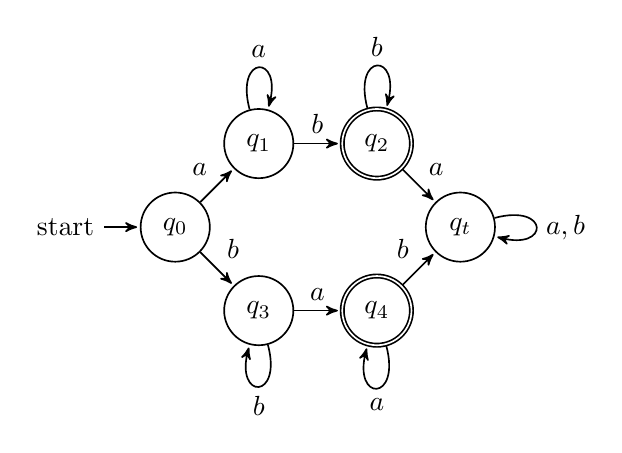
\begin{tikzpicture}[->,>=stealth',shorten >=1pt,auto,node distance=1.5cm,
                              semithick]

        \node[state,initial] (q0) {$q_{0}$};
        \node[state] (q1) [above right of=q0] {$q_{1}$};
        \node[state,accepting] (q2) [right of=q1] {$q_{2}$};
        \node[state] (q3) [below right of=q0] {$q_{3}$};
        \node[state,accepting] (q4) [right of=q3] {$q_{4}$};

        \node[state] (t)  [below right of=q2] {$q_{t}$};

        \path (q0) edge [->] node {$a$} (q1)
                   edge [->] node {$b$} (q3)
              (q1) edge [->, loop above] node {$a$} (q1)
                   edge [->] node {$b$} (q2)
              (q2) edge [->] node {$a$} (t)
                   edge [->, loop above] node {$b$} (q2)
              (q3) edge [->] node {$a$} (q4)
                   edge [->, loop below] node {$b$} (q3)
              (q4) edge [->, loop below] node {$a$} (q4)
                   edge [->] node {$b$} (t)
              (t)  edge [->, loop right] node {$a,b$} (t);
      \end{tikzpicture}
    \end{figure}
    The automaton $\mathfrak{A}$ does both, Büchi- and co-Büchi-recognize $L$.


  \subsection*{b}
    Assume $\mathfrak{A}^{\prime}$ E-recognizes $L$. So for $\rho (i)=q_{f}$ and
    $q_{f}\in F$ for $i \in \mathbb{N}$. So the read letter before the accepting
    state is reached are final. Let the read word be $w=a^{1+n_1}b^{n_2}$. So
    $\mathfrak{A}^\prime$ would recognize $w$ but $w\not\in L$. Contradiction 
    $\mathfrak{A}^{\prime}$ does not recognize $L$.

    Assume $\mathfrak{A}^{\prime\prime}$ A-recognizes $L$. Let
    $w=a^{u}b^{\omega}$. So $\rho(i)=q_{f}$ where $q_{f}\in F$ and $i\leq u$. By
    repeating the letter $a$ the automaton must allways reach a final state. So
    $w=a^\omega$ leads to a final state. This means $\mathfrak{A}^{\prime\prime}$
    recognizes $w=a^\omega \not\in L$. Contradiction $\mathfrak{A}^{\prime\prime}$
    does not recognize $L$.

  \newpage
  \subsection*{c}
    $\mathfrak{A}_{A}:$
    \begin{figure}[h]
      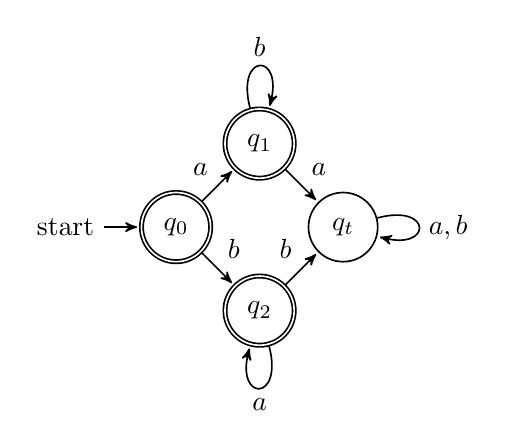
\begin{tikzpicture}[->,>=stealth',shorten >=1pt,auto,node distance=1.5cm,
                              semithick]

        \node[state,accepting,initial] (q0) {$q_{0}$};
        \node[state,accepting] (q1) [above right of=q0] {$q_{1}$};
        \node[state,accepting] (q2) [below right of=q0] {$q_{2}$};

        \node[state] (t)  [below right of=q1] {$q_{t}$};

        \path (q0) edge [->] node {$a$} (q1)
                   edge [->] node {$b$} (q2)
              (q1) edge [->, loop above] node {$b$} (q1)
                   edge [->] node {$a$} (t)
              (q2) edge [->] node {$b$} (t)
                   edge [->, loop below] node {$a$} (q2)
              (t)  edge [->, loop right] node {$a,b$} (t);
      \end{tikzpicture}
    \end{figure}

\section*{Exercise 28}
  \subsection*{a}
    $\mathfrak{A}_{SW}:$
    \begin{figure}[h]
      \begin{tikzpicture}[->,>=stealth',shorten >=1pt,auto,node distance=3cm,
                              semithick]

        \node[state,initial] (q0) {$q_{0}$};
        \node[state] (q2) at (2,0)  {$q_{1}$};
        \node[state] (q1) at (2+\Xdist,\Ydist)  {$q_{2}$};
        \node[state] (q3) at (2+\Xdist, -\Ydist)  {$q_{3}$};


        \path (q0) edge [->,bend left] node {$a$} (q1)
                   edge [->] node {$b$} (q2)
                   edge [->,bend right] node {$c$} (q3)
              (q1) edge [->,loop above] node {$a$} (q1)
                   edge [->,bend right] node {$b$} (q2)
                   edge [->,bend right] node {$c$} (q3)
              (q2) edge [->,bend right] node {$a$} (q1)
                   edge [->, loop below] node {$b$} (q2)
                   edge [->,bend right] node {$c$} (q3)
              (q3) edge [->,bend right] node {$a$} (q1)
                   edge [->,bend right] node {$b$} (q2)
                   edge [->,loop right] node {$c$} (q3)
                   ;
      \end{tikzpicture}
    \end{figure}

    $\mathcal{F}=\{\{q_{0}\}, \{q_{0},q_{2}\}, \{q_{0},q_{3}\},
    \{q_{0},q_{1},q_{3}\}, \{q_{0},q_{2},q_{3}\}, \{q_{0},q_{1},q_{2},q_{3}\} \}$

  \newpage
  \subsection*{b}
    $\mathfrak{A}_{SW}^{\prime}:$
    \begin{figure}[h]
      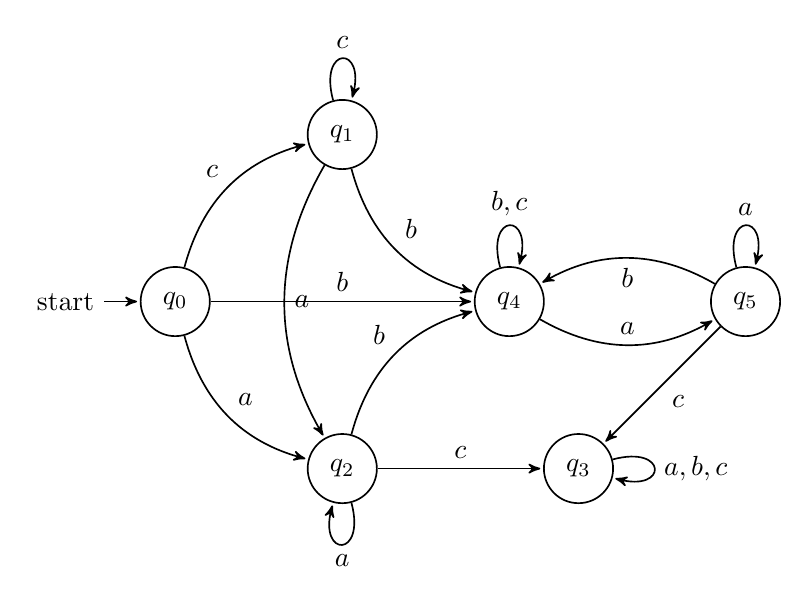
\begin{tikzpicture}[->,>=stealth',shorten >=1pt,auto,node distance=3cm,
                              semithick]

        \node[state,initial] (q0) {$q_{0}$};
        \node[state] (q1) [above right of=q0] {$q_{1}$};
        \node[state] (q2) [below right of=q0] {$q_{2}$};
        \node[state] (q3) [right of=q2] {$q_{3}$};
        \node[state] (q4) [above right of=q2] {$q_{4}$};
        \node[state] (q5) [right of=q4] {$q_{5}$};


        \path (q0) edge [->,bend left] node {$c$} (q1)
                   edge [->,bend right] node {$a$} (q2)
                   edge [->] node {$b$} (q4)
              (q1) edge [->,loop above] node {$c$} (q1)
                   edge [->,bend right] node {$b$} (q4)
                   edge [->,bend right] node {$a$} (q2)
              (q2) edge [->,loop below] node {$a$} (q1)
                   edge [->,bend left] node {$b$} (q4)
                   edge [->] node {$c$} (q3)
              (q3) edge [->,loop right] node {$a,b,c$} (q3)
              (q4) edge [->,loop above] node {$b,c$} (q4)
                   edge [->,bend right] node {$a$} (q5)
              (q5) edge [->,loop above] node {$a$} (q5)
                   edge [->,bend right] node {$b$} (q4)
                   edge [->] node {$c$} (q3)
                   ;
      \end{tikzpicture}
    \end{figure}

    $\mathcal{F}=\{ \\
      \{q_0\}, \\
      \{q_0,q_1\}, \{q_0, q_2\}, \{q_0,q_4\}, \\
      \{q_0,q_1,q_2\}, \{q_0,q_1,q_4\}, \{q_0,q_2,q_4\}, \{q_0,q_4,q_5\}, \\
      \{q_0,q_1,q_2,q_4\}, \{q_0,q_1,q_4,q_5\},\{q_0,q_2,q_4,q_5\}, \\
      \{q_0,q_1,q_2,q_4,q_5\} \\
      \}$

    
      

\end{document}

